\section{Acompanhar Lançamentos}

\subsection{Caso de uso descritivo}

Este caso de uso tem como função permitir que o usuário consiga acompanhar os lançamentos realizados em sua conta.

\begin{table}[h]
  \centering
  \begin{tabular}{|p{4cm} | p{10cm} |}
      \hline
      \small{\textbf{Requisitos Não Funcionais Associados}}	&	Tempo de acesso, segurança, interface amigável e acessível	\\ \hline
      \small{\textbf{Pré-condição}}	&	O usuário deve ser cliente do banco e deve possuir uma conta ativa	\\ \hline
      \small{\textbf{Pós-condição}}	&	O usuário visualiza os lançamentos realizados de acordo com o filtro aplicado	\\ \hline
    \end{tabular}
 \captionof{table}{Condições para o caso de uso Acompanhar Lançamentos}
\end{table}

\textbf{Fluxo de eventos principal:}

\begin{enumerate}
  \item O usuário acessa o sistema utilizando suas credenciais.
  \item O sistema realiza a validação dos dados informados.
  \item O usuário seleciona a opção ``Lançamentos da minha conta''.
  \item O sistema exibe opções de filtros a serem aplicados nos lançamentos.
  \item O usuário seleciona a opção ``Todos os lançamentos''.
  \item O sistema solicita o levantamento dos lançamentos da conta do usuário.
  \item Ao obter os dados dos lançamentos da conta do usuário, o sistema retorna os lançamentos para a tela, informando os lançamentos de acordo com o filtro aplicado.
\end{enumerate}

\textbf{Fluxos secundários:}

\begin{itemize}
  \item \textbf{Fluxo secundário – Acompanhar lançamentos no modo débito}

  No passo 5 do fluxo de eventos principal:
  \subitem Se o usuário selecionar ``Lançamentos no modo débito'', só serão exibidos os lançamentos referentes ao modo débito.

  \item \textbf{Fluxo secundário – Acompanhar lançamentos no modo crédito}

  No passo 5 do fluxo de eventos principal:
  \subitem Se o usuário selecionar ``Lançamentos no modo débito'', só serão exibidos os lançamentos referentes ao modo crédito.
\end{itemize}

\subsection{Diagrama de caso de uso}

\begin{figure}[!htb]
     \centering
     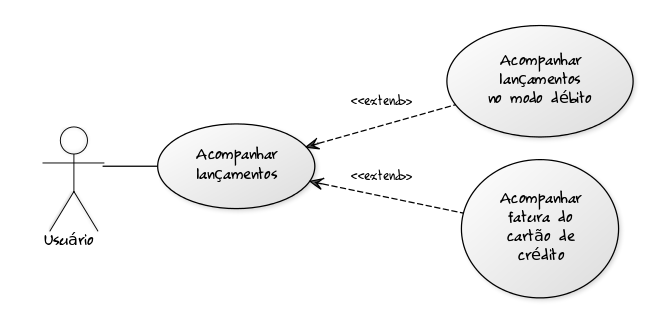
\includegraphics[scale=0.6]{diagramas/caso-de-uso/imagens/acompanharLancamento.png}
     \caption{Caso de uso Acompanhar Lançamento}
\end{figure}

\subsection{Diagrama de classes para o caso de uso}

\section{Realizar compra no cartão de crédito}

\subsection{Caso de uso descritivo}

Este caso de uso tem como função permitir que o usuário consiga realizar uma compra utilizando seu cartão de crédito.

\begin{table}[h]
  \centering
  \begin{tabular}{|p{4cm} | p{10cm} |}
      \hline
      \small{\textbf{Requisitos Não Funcionais Associados}}	&	Tempo de validação e segurança	\\ \hline
      \small{\textbf{Pré-condição}}	&	O usuário deve ser cliente do banco, possuir uma conta ativa e possuir saldo suficiente na fatura para realizar a compra	\\ \hline
      \small{\textbf{Pós-condição}}	&	A compra é realizada com sucesso e o valor da fatura é acrescido do valor da compra	\\ \hline
    \end{tabular}
 \captionof{table}{Condições para o caso de uso Realizar compra no cartão de crédito}
\end{table}

\textbf{Fluxo de eventos principal:}

\begin{enumerate}
  \item O usuário visita um site de compras e realiza uma compra via cartão de crédito.
  \item O usuário informa os dados do cartão de crédito e permite a cobrança.
  \item O sistema do site de compras envia os dados para o sistema de integração do banco.
  \item O sistema do banco valida os dados.
  \item O sistema verifica se o cliente possui saldo suficiente na sua fatura para realizar a compra.
  \item O sistema concede a cobrança, aumentando assim o valor de sua fatura atual.
  \item O sistema bancário retorna uma resposta de sucesso para o site de compras.
\end{enumerate}

\textbf{Fluxos secundários:}

\begin{itemize}
  \item \textbf{Fluxo secundário – Realizar compra com cartão físico}

  No passo 1, 2 e 3 do fluxo de eventos principal:
  \subitem O usuário vai até uma loja e realiza uma compra com o modo de pagamento cartão de crédito.
  \subitem O usuário insere seu cartão na máquina leitora de cartões e digita sua senha.
  \subitem A máquina leitora envia os dados para o sistema de integração do banco.

  Após o passo 8 do fluxo de eventos principal:
  \subitem A máquina leitora, ao receber a resposta de sucesso exibe a mensagem sucesso ao operador e imprimindo o comprovante.


\end{itemize}

\subsection{Diagrama de caso de uso}

\begin{figure}[!htb]
     \centering
     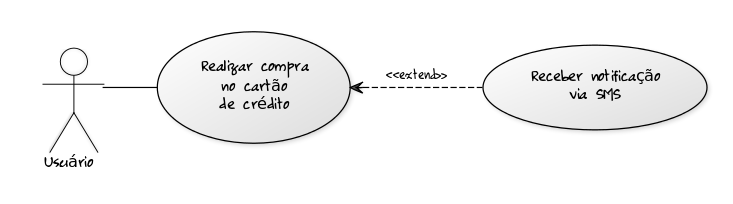
\includegraphics[scale=0.6]{diagramas/caso-de-uso/imagens/realizarCompraCartao.png}
     \caption{Caso de uso Realizar compra no cartão de crédito}
\end{figure}

\subsection{Diagrama de classes para o caso de uso}

\section{Bloquear cartão}

\subsection{Caso de uso descritivo}

Este caso de uso tem como função permitir que o usuário consiga bloquear o cartão associado a sua conta.

\begin{table}[h]
  \centering
  \begin{tabular}{|p{4cm} | p{10cm} |}
      \hline
      \small{\textbf{Requisitos Não Funcionais Associados}}	&	Tempo de acesso, segurança, interface amigável e acessível	\\ \hline
      \small{\textbf{Pré-condição}}	&	O usuário deve ser cliente do banco e deve possuir uma conta ativa	\\ \hline
      \small{\textbf{Pós-condição}}	&	O usuário terá o cartão bloqueado e não poderá utilizá-lo para movimentações bancárias	\\ \hline
    \end{tabular}
 \captionof{table}{Condições para o caso de uso Bloquear cartão}
\end{table}

\textbf{Fluxo de eventos principal:}

\begin{enumerate}
  \item O usuário acessa o sistema utilizando suas credenciais.
  \item O sistema realiza a validação dos dados informados.
  \item O usuário seleciona a opção ``Cartões''.
  \item O sistema exibe opções de cartões referentes a conta.
  \item O usuário seleciona o cartão desejado.
  \item O sistema exibe as opções disponíveis para o cartão selecionado.
  \item O usuário seleciona a opção ``Bloquear cartão''.
  \item O sistema solicita as credenciais do usuário para confirmação do bloqueio do cartão.
  \item O usuário insere as credenciais.
  \item O sistema realiza a validação dos dados informados.
  \item O sistema retorna uma mensagem informando que o cartão foi bloqueado.
\end{enumerate}

\subsection{Diagrama de caso de uso}

\begin{figure}[!htb]
     \centering
     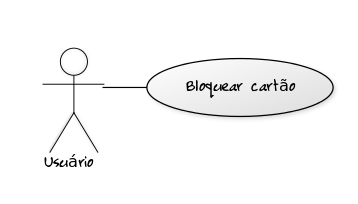
\includegraphics[scale=0.6]{diagramas/caso-de-uso/imagens/bloquearCartao.png}
     \caption{Caso de uso Bloquear cartão}
\end{figure}

\subsection{Diagrama de classes para o caso de uso}
